\chapter{البوزونات المركبة، وتمثيلات اللف المغزلي، ومضاعفة ديراك}

\section{تناظر التبادل والبوزونات المركبة}

السؤال الافتتاحي مفارقة حقيقية تتعلق بالجسيمات المركبة. فإذا كان فرميونان يؤلفان بوزونًا، فهل يمكن لبوزونين من هذا النوع أن يشغلا الحالة نفسها من دون انتهاك استبعاد الفرميونات؟ تبدأ الإجابة من قاعدة التبادل نفسها.

افترض أن جسيمين متماثلين توصفهما دالة موجية ذات متغيرين. يوسم الرمزان \(x\) و\(y\) خانتي الجسيمين؛ وهما لا يميزان بين نوعين مختلفين. بالنسبة إلى البوزونات تكون الدالة الموجية متناظرة، بينما تكون بالنسبة إلى الفرميونات متضادة التناظر:
\begin{equation}
\Psi_B(x,y)=\Psi_B(y,x),
\qquad
\Psi_F(x,y)=-\Psi_F(y,x).
\end{equation}
ويعني هذا التناظر أن تبديل الجسيمين غير القابلين للتمييز لا ينتج حالة فيزيائية جديدة.

يمكن بالتأكيد لبوزونين أن يشغلا الحالة نفسها لجسيم واحد. وإذا كانت لتلك الحالة الدالة الموجية \(\varphi\)، فإن حاصل الضرب ذي الجسيمين هو
\begin{equation}
\Psi(x,y)=\varphi(x)\varphi(y).
\end{equation}
الدوال الموجية دوال اعتيادية ذات قيم عقدية، وليست مؤثرات ولا مصفوفات، لذا فإن قيمها تبديلية:
\begin{equation}
\varphi(x)\varphi(y)=\varphi(y)\varphi(x).
\end{equation}
ولذلك يكون حاصل الضرب متناظرًا. ولا يمكن للبناء نفسه أن يعطي حالة غير صفرية لفرميونين، لأن التضاد في التناظر يقتضي
\begin{equation}
\varphi(x)\varphi(y)=-\varphi(y)\varphi(x),
\end{equation}
في حين أن الطرفين، من دون إشارة السالب، متساويان.

وعلى نحو أعم، ابدأ بأي دالة موجية لجسيمين \(F(x,y)\)، من دون افتراض أي تناظر تبادل لها. وجزآها المتناظر والمتضاد التناظر هما، باستثناء عامل التطبيع،
\begin{align}
F_{\mathrm{sym}}(x,y)&=F(x,y)+F(y,x),\\
F_{\mathrm{asym}}(x,y)&=F(x,y)-F(y,x).
\end{align}
والتحقق من التبادل صريح:
\begin{align}
F_{\mathrm{sym}}(y,x)
&=F(y,x)+F(x,y)
=F_{\mathrm{sym}}(x,y),\\
F_{\mathrm{asym}}(y,x)
&=F(y,x)-F(x,y)
=-F_{\mathrm{asym}}(x,y).
\end{align}
إن إضافة الدالة المبدلة تجعلها متناظرة؛ وطرح الدالة المبدلة يجعلها متضادة التناظر.

يوفر زوج من ذرات الهيدروجين الحالة الأكثر إثارة للاهتمام. فهناك أربعة فرميونات مكوِّنة: إلكترونان متماثلان وبروتونان متماثلان. ولتكن \(x_1,x_2\) دالة على متغيرات الإلكترونين، و\(y_1,y_2\) على متغيرات البروتونين. ويجب أن تكون الدالة الموجية رباعية الأجسام متضادة التناظر على نحو منفصل تحت تبادل الإلكترونين وتحت تبادل البروتونين:
\begin{align}
\Psi(x_2,x_1;y_1,y_2)
&=-\Psi(x_1,x_2;y_1,y_2),\\
\Psi(x_1,x_2;y_2,y_1)
&=-\Psi(x_1,x_2;y_1,y_2).
\end{align}

وللتمهيد لدالتين موجيتين متميزتين لذرة واحدة، تخيل ذرة هيدروجين متمركزة قرب الأصل، ذات دالة موجية \(\psi(x,y)\)، وأخرى متمركزة في موضع آخر، ذات دالة موجية \(\phi(x,y)\). وقد تكون الثانية ببساطة نسخة مزاحة من الأولى، تُستحصل بإزاحة وسيطي الإلكترون والبروتون فيها معًا، لكنها مع ذلك دالة موجية متميزة في هذا الإعداد. وحاصل ضرب ساذج هو
\begin{equation}
\psi(x_1,y_1)\phi(x_2,y_2).
\end{equation}
وهو لا يملك بعد أيًّا من خاصيتي التضاد الفرميوني المطلوبتين.

أولًا اجعل متغيرات الإلكترون متضادة التناظر:
\begin{equation}
\Psi_x=
\psi(x_1,y_1)\phi(x_2,y_2)
-\psi(x_2,y_1)\phi(x_1,y_2).
\end{equation}
تحت \(x_1\leftrightarrow x_2\)، يتبادل الحدان موضعيهما وتتغير إشارة التعبير كله. والآن اجعل هذه النتيجة متضادة التناظر في متغيرات البروتون. ويتحدد ترتيب الحدود الأربعة بعمليتي جعل التضاد في التناظر المتعاقبتين.\footnote{ويحدد هذا البناء أيضًا نمط الإشارات \(+,-,-,+\) من خلال تصحيحات وسوم المتغيرات التي أُجريت أثناء الحساب الشفهي.}
\begin{align}
\Psi_{2H}(x_1,x_2;y_1,y_2)
&=\Psi_x(x_1,x_2;y_1,y_2)\nonumber\\
&\quad{}-\Psi_x(x_1,x_2;y_2,y_1)\\
&=\psi(x_1,y_1)\phi(x_2,y_2)\nonumber\\
&\quad{}-\psi(x_2,y_1)\phi(x_1,y_2)\nonumber\\
&\quad{}-\psi(x_1,y_2)\phi(x_2,y_1)\nonumber\\
&\quad{}+\psi(x_2,y_2)\phi(x_1,y_1).
\label{eq:two-hydrogen-antisymmetrized}
\end{align}
إن تبادل إلكترونين يبدل الحدين الأول والثاني، والحدين الثالث والرابع، مع انقلاب في الإشارة الكلية. ويفعل تبادل البروتونين الشيء نفسه. ومن ثم تمتلك الحالة بالضبط خاصيتي التضاد المنفصلتين المطلوبتين لفرميونات المكوِّنات.

\begin{classroomqa}
\lecturetimestamp{00:11:11}
\audiencequestion{إذا كانت ذرات الهيدروجين بوزونات، فما الذي يمنع وضع اثنتين منها مباشرة فوق بعضهما؟}
\lecturerresponse{إحصاء التبادل البوزوني لا يزيل القوى بين الذرات. ويمكن لاستبعاد باولي بين المكوِّنات، مع القوى الأخرى بين الذرات، أن يجعل التراكب المكاني باهظ الكلفة جدًا. وهذا يختلف عن السؤال عما إذا كان يجوز للذرات أن تشغل حالة الزخم اللاموضعية نفسها. فالحالة الذاتية للزخم منتشرة في الفضاء كله، لذا فإن اشتراك الذرات في الزخم لا يعني دفعها إلى النقطة نفسها. وحتى الأجسام ذات اللب الصلب مثل كرات البلياردو يمكن أن تخضع لإحصاء تبادل بوزوني: فلبابها الصلبة تمنع التراكب المكاني، بينما يظل الإحصاء البوزوني يسمح بإشغال حالة الزخم نفسها.}
\end{classroomqa}

\begin{classroomqa}
\lecturetimestamp{00:12:28}
\audiencequestion{هل إن وضع ذرتي هيدروجين في الحالة الذاتية نفسها للزخم يضع فرميوناتهما المكوِّنة في الحالة نفسها؟}
\lecturerresponse{لا. تظل الحالة رباعية الأجسام متضادة التناظر تحت تبادل متغيري الإلكترونين، ومتضادة التناظر على نحو منفصل تحت تبادل متغيري البروتونين. أما التبادل المتزامن لكلا المكوِّنين---أي تبادل الذرتين الكاملتين---فهو وحده المتناظر.}
\end{classroomqa}

في الواقع، إن تبديل الذرتين يعني إجراء الاستبدالين معًا
\begin{equation}
x_1\leftrightarrow x_2,
\qquad
y_1\leftrightarrow y_2.
\end{equation}
يسهم الاستبدال الأول بإشارة سالب فرميونية واحدة، ويسهم الثاني بأخرى:
\begin{equation}
\begin{aligned}
\Psi_{2H}(x_2,x_1;y_2,y_1)
&=(-1)(-1)\Psi_{2H}(x_1,x_2;y_1,y_2)\\
&=\Psi_{2H}(x_1,x_2;y_1,y_2).
\end{aligned}
\end{equation}
ويمكن رؤية النتيجة نفسها حدًا فحدًا في المعادلة~\eqref{eq:two-hydrogen-antisymmetrized}. فعند تبادل الذرتين الكاملتين،
\begin{equation}
\psi(x_1,y_1)\phi(x_2,y_2)
\longleftrightarrow
\psi(x_2,y_2)\phi(x_1,y_1),
\end{equation}
ومن ثم يتبادل الحدان الأول والرابع. وبالمثل،
\begin{equation}
-\psi(x_2,y_1)\phi(x_1,y_2)
\longleftrightarrow
-\psi(x_1,y_2)\phi(x_2,y_1),
\end{equation}
ومن ثم يتبادل الحدان الثاني والثالث. والحالة الكاملة متناظرة تحت تبديل الذرتين. إن إشارتَي السالب الآتيتين من المكوِّنين تعطيان المركب إشارة موجبة.

هذا الحكم المتعلق بالتبادل مستقل منطقيًا عن الطاقة اللازمة لتراكب الذرات. فقد يجعل التنافر الشديد مثل هذا التراكب متعذر المنال، لكنه لا يغير قانون التبادل المتناظر.

\begin{classroomqa}
\lecturetimestamp{00:14:42}
\audiencequestion{ماذا تمثل فيزيائيًا الحالة رباعية الأجسام المبنية هنا، وهل هي على التحديد حالة في فضاء الزخم؟}
\lecturerresponse{إنها الدالة الموجية لذرتين، المستحصلة من دالتين موجيتين لذرة واحدة بجعل وسوم الإلكترون أولًا متضادة التناظر ثم وسوم البروتون. ولا يلزم أن تكون مكتوبة في فضاء الزخم. فقد تصف المتغيرات الموضع أو الزخم أو تمثيلًا آخر؛ وتناظرات التبادل المطلوبة للمكوِّنات هي نفسها.}
\end{classroomqa}

وبالتالي، قد تشغل ذرتان الدالة الموجية نفسها لحالة زخم لا موضعية، رغم أن إجبار توزيعيهما المكانيين على تراكب قوي قد يكلّف قدرًا كبيرًا من الطاقة.

الآن اجعل الدالتين الموجيتين لذرة واحدة متساويتين، \(\phi=\psi\). تصبح المعادلة~\eqref{eq:two-hydrogen-antisymmetrized}
\begin{align}
\Psi_{\mathrm{same}}
&=\psi(x_1,y_1)\psi(x_2,y_2)
-\psi(x_2,y_1)\psi(x_1,y_2)\nonumber\\
&\quad
-\psi(x_1,y_2)\psi(x_2,y_1)
+\psi(x_2,y_2)\psi(x_1,y_1).
\end{align}

هل تنعدم هذه الحالة رباعية الأجسام؟ لا، لا تنعدم. فحاصل الضرب الأول والرابع متساويان، والثاني والثالث متساويان. وباستخدام تبديلية الدوال الموجية لذرة واحدة،
\begin{equation}
\Psi_{\mathrm{same}}
=
2\left[
\psi(x_1,y_1)\psi(x_2,y_2)
-\psi(x_2,y_1)\psi(x_1,y_2)
\right],
\label{eq:same-hydrogen-state}
\end{equation}
وهو غير صفري عمومًا. وتبقى متضادة التناظر في متغيري الإلكترونين، ومتضادة التناظر على نحو منفصل في متغيري البروتونين.

لا يوجد هنا إسناد لإلكترون محدد الموضع بدقة إلى كل ذرة محددة الموضع بدقة. فالإلكترون المرتبط في ذرة يكون لا موضعيًا مكانيًا على امتداد دالته الموجية الذرية. لذا فإن إعطاء الذرتين الحالة الذرية نفسها لا يفرض \(x_1=x_2\)، ولا يفرض \(y_1=y_2\).

يظهر استبعاد المكوِّنات باختبار التطابق مباشرة. فإذا تطابق متغيرا الإلكترونين الممثلان، \(x_1=x_2=x\)، فإن المعادلة~\eqref{eq:same-hydrogen-state} تعطي
\begin{align}
\Psi_{\mathrm{same}}(x,x;y_1,y_2)
&=2\bigl[
\psi(x,y_1)\psi(x,y_2)\nonumber\\
&\quad{}-\psi(x,y_1)\psi(x,y_2)
\bigr]\\
&=0.
\end{align}
وينعدم التعبير المناظر أيضًا عندما \(y_1=y_2\). وهكذا تكون الدالة الموجية المركبة للحالة نفسها غير صفرية، بينما تنعدم سعتها عند تطابق متغيرات الفرميونات المتماثلة.\footnote{حُذِف في هذا النموذج اللف المغزلي وأي وسوم أخرى لجسيم واحد. وينطبق التضاد الفرميوني في التناظر على المجموعة الكاملة من وسوم الجسيم الواحد؛ أما الإلغاء المعروض هنا فيتعلق بتطابق المتغيرات المحتفَظ بها هنا.}

\begin{classroomqa}
\lecturetimestamp{00:20:41}
\audiencequestion{هل يمكن أن تكون الذرات في الحالة نفسها بينما لا تكون إلكتروناتها وبروتوناتها في حالات المكوِّنات نفسها؟}
\lecturerresponse{نعم. فمساواة الدوال الموجية الذرية المركبة لا تزيل تضادي التناظر المنفصلين للإلكترون والبروتون. ويمكن للحالة الكاملة رباعية الأجسام أن تصف ذرتين في حالة ذرية واحدة، مع إسناد سعة صفرية لمتغيرات الفرميونات المتماثلة المتطابقة.}
\end{classroomqa}

\begin{classroomqa}
\lecturetimestamp{00:21:12}
\audiencequestion{هل أسقطت عملية جعل التضاد في التناظر الأجزاء التي تتطابق فيها المكوِّنات المتماثلة؟}
\lecturerresponse{نعم. ففي المتغيرات المعروضة هنا، تُلغى تلك المكوّنات التطابقية إلغاءً تامًا. والعبارة الدقيقة هي أن الدالة الموجية المتضادة التناظر تنعدم عندما تتساوى وسيطا الفرميونين المتماثلين.}
\end{classroomqa}

لم يعتمد هذا الإلغاء على جعل الدوال الموجية الذرية متساوية أولًا. فبالنسبة إلى الحالة العامة في المعادلة~\eqref{eq:two-hydrogen-antisymmetrized}،
\begin{align}
\Psi_{2H}(x,x;y_1,y_2)
&=\psi(x,y_1)\phi(x,y_2)\nonumber\\
&\quad{}-\psi(x,y_1)\phi(x,y_2)\nonumber\\
&\quad{}-\psi(x,y_2)\phi(x,y_1)\nonumber\\
&\quad{}+\psi(x,y_2)\phi(x,y_1)\\
&=0.
\end{align}

\begin{classroomqa}
\lecturetimestamp{00:21:32}
\audiencequestion{هل يبقى هذا الإلغاء قائمًا عندما تكون الذرات في حالات مختلفة وتتطابق متغيرات المكوِّنات المتماثلة؟}
\lecturerresponse{نعم. فهو ينتج من التضاد في التناظر نفسه، لا من فرض \(\phi=\psi\). وتصح العبارة نفسها في تمثيل آخر: فبعد التحويل إلى فضاء الزخم، تنعدم السعة عندما تتطابق متغيرات الزخم لفرميونين متماثلين، بشرط أن تتطابق أيضًا وسوم الجسيم الواحد الأخرى المحذوفة.}
\end{classroomqa}

\section{اللف المغزلي بوصفه نظامًا كموميًا محدود الأبعاد}

تتكرر رياضيات اللف المغزلي في الإيزوسبين واللون وسائر التناظرات الداخلية في فيزياء الجسيمات. وهذا التشابه صوري: إذ يظهر الجبر نفسه، وإن لم يكن من الضروري أن يكون للكميات الفيزيائية التفسير نفسه. والمهمة المباشرة هي تطوير موضوع اللف المغزلي قليلًا ثم العودة إلى معادلة ديراك. وستُستخدم هذه الأدوات لاحقًا في الإيزوسبين، وهو مفهوم ارتبط تاريخيًا بسنوات 1930.

الإلكترون جسيم ذو لف مغزلي \(\tfrac12\)، وكذلك البروتون والميون. ولمركبته \(z\) من اللف المغزلي قيمتان ممكنتان. وقبل تثبيت الوحدات نكتب
\begin{equation}
S_z=m\hbar.
\end{equation}
ومن الآن فصاعدًا \(\hbar=1\). ويُخصَّص الحرف \(L\) اصطلاحًا للعزم الزاوي المداري، لذا سيُرمز إلى اللف المغزلي الذاتي بـ \(S\). وهو يحقق جبر العزم الزاوي نفسه:
\begin{equation}
[S_x,S_y]=iS_z,
\quad
[S_y,S_z]=iS_x,
\quad
[S_z,S_x]=iS_y,
\end{equation}
وكذلك
\begin{equation}
S_\pm=S_x\pm iS_y.
\end{equation}
يرفع المؤثر \(S_+\) القيمة الذاتية لـ \(S_z\)، ويخفضها \(S_-\).

\begin{classroomqa}
\lecturetimestamp{00:25:39}
\audiencequestion{هل يدور النقاش تحديدًا حول اللف المغزلي الذاتي؟}
\lecturerresponse{المقصود هو التركيز على اللف المغزلي الذاتي. وينطبق جبر العزم الزاوي نفسه على نحو أعم، بما في ذلك العزم الزاوي المداري أو دوران جسم عياني.}
\end{classroomqa}

بالنسبة إلى اللف المغزلي النصفي، فإن القيم الذاتية الوحيدة لـ \(S_z\) هي \(+\tfrac12\) و\(-\tfrac12\). ولنُهمِل مؤقتًا كل ما عدا ذلك في الإلكترون: ننسى موضعه وزخمه ونحتفظ فقط بحالتي اللف المغزلي. عندئذٍ
\begin{equation}
|\psi\rangle
=
\alpha|\uparrow_z\rangle+\beta|\downarrow_z\rangle
\quad\longleftrightarrow\quad
\begin{pmatrix}
\alpha\\
\beta
\end{pmatrix},
\end{equation}
حيث
\begin{equation}
|\alpha|^2=P(\uparrow_z),
\qquad
|\beta|^2=P(\downarrow_z),
\qquad
|\alpha|^2+|\beta|^2=1.
\end{equation}
هذا فضاء حالات ثنائي الأبعاد. وليس في ذلك ادعاء بأن الفضاء العادي ثنائي الأبعاد.

\begin{classroomqa}
\lecturetimestamp{00:28:18}
\audiencequestion{هل قيل إن الفضاء الفيزيائي ثنائي الأبعاد؟}
\lecturerresponse{لا. فضاء حالات اللف المغزلي ثنائي الأبعاد. وقد أُهمِل الموضع والزخم مؤقتًا، كما لو كان الإلكترون مُثبَّتًا إلى جدار ولا يمكن قياس إلا لفه المغزلي.}
\end{classroomqa}

تُمثَّل المؤثرات على فضاء الحالات هذا بمصفوفات \(2\times2\). ومن الملائم اختيار قاعدة \(S_z\) بحيث يكون \(S_z\) قطريًا، لكن القطرية اختيار للقاعدة لا متطلب فيزيائي.

\begin{classroomqa}
\lecturetimestamp{00:29:46}
\audiencequestion{هل يجب أن يكون \(S_z\) قطريًا؟}
\lecturerresponse{لا. يُختار قطريًا تيسيرًا للحساب. والتمثيلات المصفوفية الأخرى مكافئة له فيزيائيًا.}
\end{classroomqa}

\begin{classroomqa}
\lecturetimestamp{00:30:08}
\audiencequestion{هل \(S_z\) مصفوفة؟}
\lecturerresponse{\(S_z\) كمية قابلة للرصد، ولذا فهو مؤثر. وفي القاعدة المختارة المحدودة البعد، يُمثَّل هذا المؤثر بمصفوفة تؤثر في متجهات الحالة.}
\end{classroomqa}

تمثيل مفيد على نحو خاص هو
\begin{equation}
S_i=\frac12\sigma_i,
\end{equation}
حيث
\begin{equation}
\sigma_x=
\begin{pmatrix}
0&1\\
1&0
\end{pmatrix},
\quad
\sigma_y=
\begin{pmatrix}
0&-i\\
i&0
\end{pmatrix},
\quad
\sigma_z=
\begin{pmatrix}
1&0\\
0&-1
\end{pmatrix}.
\end{equation}
المصفوفات من دون عامل النصف هي مصفوفات باولي؛ أما مؤثرات اللف المغزلي نفسها فتتضمن هذا العامل. ويؤكد الضرب المباشر علاقات التبادل. والتمثيل غير فريد: فإدارة المحاور أو تغيير القاعدة ينتج ثلاثية أخرى مكافئة.

هذا تمثيل ثنائي المركبتين للعزم الزاوي ذي اللف المغزلي النصفي.

\subsection{الحالات الذاتية على امتداد المحاور الإحداثية}

من المفيد حل معادلات القيم الذاتية مركبةً مركبةً. وبما أن القيم الذاتية لـ \(\sigma_i\) هي \(\pm1\)، فإن القيم الذاتية لـ \(S_i=\sigma_i/2\) هي \(\pm\tfrac12\).

بالنسبة إلى \(\sigma_z\)، فالمعادلتان هما
\begin{align}
\begin{pmatrix}
1&0\\
0&-1
\end{pmatrix}
\begin{pmatrix}
\alpha\\
\beta
\end{pmatrix}
&=
\begin{pmatrix}
\alpha\\
\beta
\end{pmatrix},
&
\begin{pmatrix}
1&0\\
0&-1
\end{pmatrix}
\begin{pmatrix}
\alpha\\
\beta
\end{pmatrix}
&=
-
\begin{pmatrix}
\alpha\\
\beta
\end{pmatrix}.
\end{align}

\begin{figure}[t]
\centering
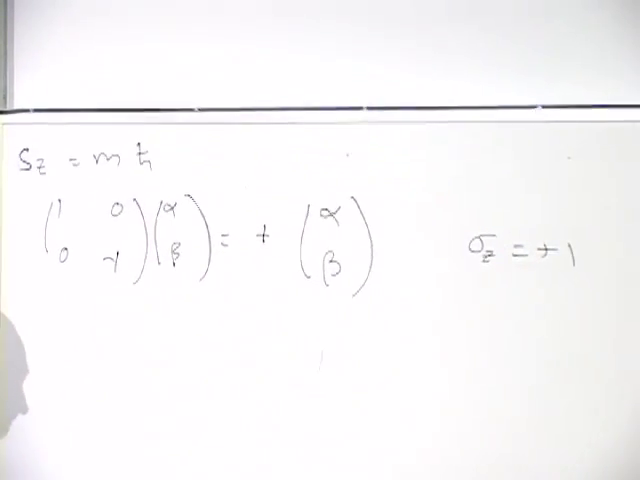
\includegraphics[width=0.74\textwidth]{lecture_08_figure_02.png}
\caption{معادلة القيمة الذاتية \(+1\) لـ \(\sigma_z\) عندما يؤثر في سبينور ذي مركبتين.}
\lectureframe{00:34:57}
\end{figure}

بالنسبة إلى القيمة الذاتية \(+1\)، فإن الضرب صفًا صفًا يعطي
\begin{equation}
\begin{pmatrix}
1\cdot\alpha+0\cdot\beta\\
0\cdot\alpha-\beta
\end{pmatrix}
=
\begin{pmatrix}
\alpha\\
-\beta
\end{pmatrix}
=
\begin{pmatrix}
\alpha\\
\beta
\end{pmatrix}.
\end{equation}
المعادلة العليا متحققة تلقائيًا، بينما تعطي السفلى \(-\beta=\beta\)، ومن ثم \(\beta=0\). ويشترط التطبيع \(|\alpha|=1\)؛ وباختيار الطور الكلي غير ذي الصلة بحيث \(\alpha=1\)،
\begin{equation}
|+z\rangle=
\begin{pmatrix}
1\\
0
\end{pmatrix}.
\end{equation}

بالنسبة إلى القيمة الذاتية \(-1\)،
\begin{equation}
\begin{pmatrix}
\alpha\\
-\beta
\end{pmatrix}
=
\begin{pmatrix}
-\alpha\\
-\beta
\end{pmatrix}.
\end{equation}
فالآن تكون المعادلة السفلى متحققة تلقائيًا، وتعطي العليا \(\alpha=-\alpha\)، ومن ثم \(\alpha=0\). وباختيار \(\beta=1\) نحصل على
\begin{equation}
|-z\rangle=
\begin{pmatrix}
0\\
1
\end{pmatrix}.
\end{equation}

الآن غيّر التجربة وقِس \(S_x\). وبما أن
\begin{equation}
\sigma_x
\begin{pmatrix}
\alpha\\
\beta
\end{pmatrix}
=
\begin{pmatrix}
0\cdot\alpha+\beta\\
\alpha+0\cdot\beta
\end{pmatrix}
=
\begin{pmatrix}
\beta\\
\alpha
\end{pmatrix},
\end{equation}
فإن معادلة \(+1\) تصبح
\begin{equation}
\begin{pmatrix}
\beta\\
\alpha
\end{pmatrix}
=
\begin{pmatrix}
\alpha\\
\beta
\end{pmatrix}.
\end{equation}
ومعادلتَا المركبتين، \(\beta=\alpha\) و\(\alpha=\beta\)، هما الشرط نفسه. ويعطي التطبيع
\begin{equation}
2|\alpha|^2=1,
\end{equation}
لذا فإن اختيارًا ملائمًا هو
\begin{equation}
|+x\rangle
=
\frac{1}{\sqrt2}
\begin{pmatrix}
1\\
1
\end{pmatrix}.
\end{equation}

\begin{figure}[t]
\centering
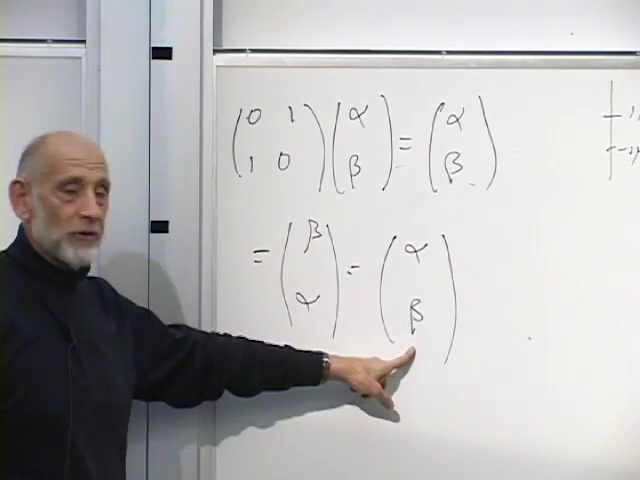
\includegraphics[width=0.74\textwidth]{lecture_08_figure_03.png}
\caption{بالنسبة إلى القيمة الذاتية \(+1\)، فإن \(\sigma_x\) يبدّل المركبتين، مما يقتضي \(\alpha=\beta\).}
\lectureframe{00:39:42}
\end{figure}

\begin{classroomqa}
\lecturetimestamp{00:40:13}
\audiencequestion{إذا أُدرج عامل النصف، فهل تكون القيمة الذاتية نصفًا؟}
\lecturerresponse{نعم. فمصفوفة باولي \(\sigma_x\) لها القيم الذاتية \(\pm1\)، بينما \(S_x=\sigma_x/2\) له القيم الذاتية \(\pm\tfrac12\).}
\end{classroomqa}

بالنسبة إلى القيمة الذاتية \(-1\)،
\begin{equation}
\begin{pmatrix}
\beta\\
\alpha
\end{pmatrix}
=
-
\begin{pmatrix}
\alpha\\
\beta
\end{pmatrix},
\end{equation}
إذًا
\begin{equation}
\beta=-\alpha,
\qquad
\alpha=-\beta.
\end{equation}
وهاتان هما، من جديد، المعادلة نفسها. وبعد التطبيع،
\begin{equation}
|-x\rangle
=
\frac{1}{\sqrt2}
\begin{pmatrix}
1\\
-1
\end{pmatrix}.
\end{equation}
وعليه فإن تراكبًا متساويًا من حالتي اللف المغزلي إلى أعلى على محور \(z\) وإلى أسفل على محور \(z\) يكون مستقطبًا على طول المحور \(x\) الموجب، بينما يكون التراكب نفسه مع إشارة سالبة نسبية مستقطبًا على طول المحور \(x\) السالب.

أما بالنسبة إلى اتجاه \(y\)،
\begin{equation}
\sigma_y
\begin{pmatrix}
\alpha\\
\beta
\end{pmatrix}
=
\begin{pmatrix}
-i\beta\\
i\alpha
\end{pmatrix}.
\end{equation}
فإن المتجهين الذاتيين المُطبَّعين هما
\begin{equation}
|+y\rangle
=
\frac{1}{\sqrt2}
\begin{pmatrix}
1\\
i
\end{pmatrix},
\qquad
|-y\rangle
=
\frac{1}{\sqrt2}
\begin{pmatrix}
1\\
-i
\end{pmatrix},
\end{equation}
وذلك حتى طور كلي. وتعطي كلتا الحالتين احتمالًا مقداره \(1/2\) لكون اللف المغزلي إلى أعلى على محور \(z\) و\(1/2\) لكونه إلى أسفل على محور \(z\). والطور النسبي \(i\)، الذي لا يظهر في هذين الاحتمالين، هو ما يميّز الاستقطاب على اتجاه \(y\) من الاستقطاب على اتجاه \(x\). كما تصف التركيبات الخطية أيضًا لفًا مغزليًا مستقطبًا على امتداد اتجاهات اعتباطية؛ ويُؤجَّل ذلك الحساب.

\begin{classroomqa}
\lecturetimestamp{00:44:22}
\audiencequestion{هل أُسنِدت إشارة مركبة \(i\) إلى القيمة الذاتية الخاطئة لـ \(\sigma_y\)؟}
\lecturerresponse{قد تكون الإشارة قد أُسنِدت فعلًا إلى القيمة الذاتية الخاطئة. والتعيين هنا غير مؤكد؛ ولا يُثبَّت هنا اعتمادًا على الذاكرة.}
\end{classroomqa}

والتحقق المباشر هو
\begin{align}
\sigma_y\frac{1}{\sqrt2}
\begin{pmatrix}
1\\
i
\end{pmatrix}
&=
\frac{1}{\sqrt2}
\begin{pmatrix}
-i\,i\\
i
\end{pmatrix}
=
\frac{1}{\sqrt2}
\begin{pmatrix}
1\\
i
\end{pmatrix},\\
\sigma_y\frac{1}{\sqrt2}
\begin{pmatrix}
1\\
-i
\end{pmatrix}
&=
\frac{1}{\sqrt2}
\begin{pmatrix}
(-i)(-i)\\
i
\end{pmatrix}
=
-\frac{1}{\sqrt2}
\begin{pmatrix}
1\\
-i
\end{pmatrix}.
\end{align}
ومن ثم فإن \(+i\) يقترن بالقيمة الذاتية \(+1\)، و\(-i\) يقترن بالقيمة الذاتية \(-1\).\footnote{يبقى التعيين الشفهي غير محسوم بعد عدة تبديلات؛ أما الإشارتان المعروضتان هنا فتتحددان بعملية ضرب المصفوفة المعروضة.} وكل حالة لف مغزلي نصفي، بما في ذلك كل حالة مستقطبة على امتداد اتجاه اعتباطي، هي تركيب خطي من \(|+z\rangle\) و\(|-z\rangle\).

\section{اللف المغزلي الواحد والسبينورات المعتمدة على الموضع}

بالنسبة إلى اللف المغزلي \(1\)، فإن القيم الممكنة لـ \(S_z\) هي \(+1,0,-1\). ومن ثم فإن فضاء الحالات ثلاثي الأبعاد. واللف المغزلي \(1\) لفٌّ صحيح ويقابل إحصاءً بوزونيًا. ونحن نبحث عن ثلاث مصفوفات \(3\times3\) تحقق مبدلات العزم الزاوي نفسها.

ويُعطى أدناه تمثيل متماثل بين الاتجاهات الإحداثية الثلاثة.\footnote{تتبع إشارة \(S_y\) المصفوفة الظاهرة قرب \(00{:}48{:}50\)، كما تتحدد أيضًا بواسطة \([S_x,S_y]=iS_z\). ومن شأن قلب تلك الإشارة أن يقلب المبدل المطلوب.}
\begin{equation}
\begin{aligned}
S_x
&=
i
\begin{pmatrix}
0&0&0\\
0&0&1\\
0&-1&0
\end{pmatrix},
&
S_y
&=
i
\begin{pmatrix}
0&0&1\\
0&0&0\\
-1&0&0
\end{pmatrix},\\
S_z
&=
i
\begin{pmatrix}
0&1&0\\
-1&0&0\\
0&0&0
\end{pmatrix}.
\end{aligned}
\end{equation}
كل مصفوفة هي \(i\) في مصفوفة حقيقية مضادة للتناظر. وتحتوي كل واحدة منها على مدخل مقداره \(1\) وآخر مقداره \(-1\)، وعلى صف وعمود منعدمَين مرتبطين بإحداثيها الخاص: الأول من أجل \(S_x\)، والثاني من أجل \(S_y\)، والثالث من أجل \(S_z\). وهذا يعطي أداة تذكّر مفيدة. وفي هذا التمثيل لا يكون \(S_z\) قطريًا.

لتكن
\begin{equation}
v=
\begin{pmatrix}
\alpha\\
\beta\\
\gamma
\end{pmatrix}.
\end{equation}
إذن
\begin{equation}
S_zv
=
\begin{pmatrix}
i\beta\\
-i\alpha\\
0
\end{pmatrix}.
\end{equation}
بالنسبة إلى القيمة الذاتية \(+1\)،
\begin{equation}
i\beta=\alpha,
\qquad
-i\alpha=\beta,
\qquad
0=\gamma.
\end{equation}
ومن ثم \(\beta=-i\alpha\) و\(\gamma=0\). ويعطي التطبيع \(2|\alpha|^2=1\)، لذا
\begin{equation}
|m=+1\rangle
=
\frac{1}{\sqrt2}
\begin{pmatrix}
1\\
-i\\
0
\end{pmatrix}.
\end{equation}
وبالنسبة إلى القيمة الذاتية \(-1\)،
\begin{equation}
i\beta=-\alpha,
\qquad
-i\alpha=-\beta,
\qquad
0=-\gamma,
\end{equation}
ومن ثم \(\beta=i\alpha\) و\(\gamma=0\)، و
\begin{equation}
|m=-1\rangle
=
\frac{1}{\sqrt2}
\begin{pmatrix}
1\\
i\\
0
\end{pmatrix}.
\end{equation}
وأخيرًا، تعطي معادلة القيمة الذاتية الصفرية \(\alpha=\beta=0\)، وتترك \(\gamma\) اعتباطيًا. وحلها المطبع هو
\begin{equation}
|m=0\rangle
=
\begin{pmatrix}
0\\
0\\
1
\end{pmatrix}.
\end{equation}
ولا توجد قيم ذاتية أخرى: فهذه المتجهات الذاتية الثلاثة تستنفد الفضاء الثلاثي الأبعاد. وليست العوامل \(1/\sqrt2\) شكلية فحسب. فالمعاملات نفسها تدخل لاحقًا في تنبؤات تجريبية كمية عندما يُطبَّق هذا الجبر على الإيزوسبين.

\begin{classroomqa}
\lecturetimestamp{00:54:10}
\audiencequestion{كيف ينبغي قراءة المدخلات العقدية لهذه المتجهات الذاتية للَّف المغزلي الواحد؟}
\lecturerresponse{بالنسبة إلى \(m=+1\) فالمركبات هي \(1/\sqrt2,-i/\sqrt2,0\)؛ وبالنسبة إلى \(m=-1\) فهي \(1/\sqrt2,i/\sqrt2,0\)؛ وبالنسبة إلى \(m=0\) فهي \(0,0,1\).}
\end{classroomqa}

توجد ثلاثيات أخرى من المصفوفات تحقق الجبر نفسه وهي مكافئة فيزيائيًا. والتمثيل المتماثل أعلاه مفيد لأنه يعامل الاتجاهات الثلاثة على السواء، وسيُستخدم مرة أخرى.

\subsection{استعادة الموضع}

والآن استعد حركة الجسيم. يتبادل اللف المغزلي مع الموضع ومع الزخم، لذا يمكن تحديد أيٍّ منهما معًا مع مركبة لف مغزلي. أما الموضع والزخم فلا يتبادلان، كما أن مركبات اللف المغزلي المختلفة لا تتبادل فيما بينها.

يُوصَف جسيم متحرك ذو لف مغزلي نصفي بسبينور يعتمد على الموضع،
\begin{equation}
\psi(x)=
\begin{pmatrix}
\psi_\uparrow(x)\\
\psi_\downarrow(x)
\end{pmatrix}.
\end{equation}
والكميتان
\begin{equation}
\rho_{\uparrow_z}(x)=|\psi_\uparrow(x)|^2,
\qquad
\rho_{\downarrow_z}(x)=|\psi_\downarrow(x)|^2
\end{equation}
هما كثافتا احتمال مشتركتان للموضع واللف المغزلي. ومجموعهما،
\begin{equation}
\rho(x)=\psi^\dagger(x)\psi(x)
=|\psi_\uparrow(x)|^2+|\psi_\downarrow(x)|^2,
\end{equation}
هو كثافة الموضع. وإذا كان معلومًا أن الجسيم قد كُشف عند \(x\)، فإن الاحتمالين الشرطيين هما
\begin{equation}
P(\uparrow_z\mid x)
=
\frac{|\psi_\uparrow(x)|^2}{\psi^\dagger(x)\psi(x)},
\qquad
P(\downarrow_z\mid x)
=
\frac{|\psi_\downarrow(x)|^2}{\psi^\dagger(x)\psi(x)},
\end{equation}
متى كان \(\rho(x)\neq0\). وهكذا يُمثَّل الإلكترون بدالة موجية مكانية ذات مركبتين، مع إمكان تغيّر سعات اللف المغزلي المحلية من موضع إلى آخر.

بالنسبة إلى جسيم متحرك ذي لف مغزلي واحد، نكتب
\begin{equation}
\phi(x)=
\begin{pmatrix}
\phi_1(x)\\
\phi_2(x)\\
\phi_3(x)
\end{pmatrix}.
\end{equation}
وعند كل نقطة في الفضاء، تُشكِّل المركبات الثلاث متجهًا في فضاء اللف المغزلي نفسه المستخدم أعلاه. وجسيمات اللف المغزلي الواحد لها لف مغزلي صحيح، وهي بوزونات.

\begin{classroomqa}
\lecturetimestamp{01:00:10}
\audiencequestion{هل تمثل \(\phi_1(x)\) نفسها احتمال النتيجة \(m=+1\) للَّف المغزلي؟}
\lecturerresponse{لا. إنها سعة في الأساس المختار ذي المركبات الثلاث. وللحصول على ناتج لف مغزلي محدد، كوِّن البرا للمتجه الذاتي المطبَّع الموافق، وأسقط الحقل عليه، ثم خذ مربع القيمة المطلقة.}
\end{classroomqa}

\begin{figure}[t]
\centering
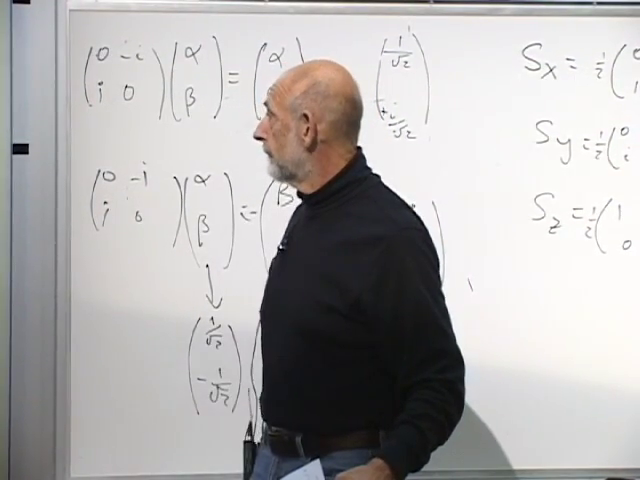
\includegraphics[width=0.82\textwidth]{lecture_08_figure_04.png}
\caption{المتجهات الذاتية المطبَّعة لـ \(\sigma_y\) إلى جانب المصفوفات الثلاث الخاصة باللف المغزلي نصف.}
\lectureframe{01:00:12}
\end{figure}

على سبيل المثال،
\begin{equation}
\begin{aligned}
|m=+1\rangle
&=
\frac{1}{\sqrt2}
\begin{pmatrix}
1\\
-i\\
0
\end{pmatrix}
\\
\Longrightarrow\quad\langle m=+1|
&=
\frac{1}{\sqrt2}
\begin{pmatrix}
1&i&0
\end{pmatrix}.
\end{aligned}
\end{equation}
ومن ثم فإن سعة الإسقاط هي
\begin{align}
\langle m=+1|\phi(x)\rangle
&=
\frac{1}{\sqrt2}
\begin{pmatrix}
1&i&0
\end{pmatrix}
\begin{pmatrix}
\phi_1(x)\\
\phi_2(x)\\
\phi_3(x)
\end{pmatrix}\\
&=
\frac{\phi_1(x)+i\phi_2(x)}{\sqrt2}.
\end{align}
ويعطي تطبيق القاعدة نفسها على المتجهات الذاتية الثلاثة كلها الكثافات المفصَّلة بحسب اللف المغزلي.\footnote{تُتم هذه الصيغ جبر الإسقاط بعد التصحيح الصريح بأن \(\phi_1\) و \(\phi_2\) ليسا بالضرورة حقيقيين. وإن معاملتهما على أنهما حقيقيان تمحو على نحو غير صحيح التداخل الذي يميز بين الكثافتين \(m=+1\) و \(m=-1\).}
\begin{align}
\rho_{+1}(x)
&=
\frac12\left|\phi_1(x)+i\phi_2(x)\right|^2,\\
\rho_{-1}(x)
&=
\frac12\left|\phi_1(x)-i\phi_2(x)\right|^2,\\
\rho_0(x)
&=
|\phi_3(x)|^2.
\end{align}
وهي تحقق
\begin{equation}
\begin{aligned}
\rho_{+1}(x)+\rho_{-1}(x)+\rho_0(x)
&=
|\phi_1(x)|^2+|\phi_2(x)|^2
\\
&\quad{}+|\phi_3(x)|^2
\\
&=
\phi^\dagger(x)\phi(x).
\end{aligned}
\end{equation}
وإذا اشترطنا أن الجسيم قد كُشف عند \(x\)، فإن
\begin{equation}
P(m\mid x)
=
\frac{\rho_m(x)}{\phi^\dagger(x)\phi(x)},
\end{equation}
بشرط \(\phi^\dagger(x)\phi(x)\neq0\). والقاعدة العامة للقياس هي دائمًا نفسها: كوِّن البرا للمتجه الذاتي المطبَّع المطلوب، وأسقط الحالة الفعلية عليه، ثم خذ مربع القيمة المطلقة. وتحتفظ الكثافة الناتجة باعتمادها على الموضع.

مصفوفات اللف الأعلى أكثر تعقيدًا، لكن المبدأ لا يتغير.

\begin{classroomqa}
\lecturetimestamp{01:07:31}
\audiencequestion{ما بُعد فضاء الحالات للَّف المغزلي ثلاثة أنصاف؟}
\lecturerresponse{له أربع حالات، مع \(m=\tfrac32,\tfrac12,-\tfrac12,-\tfrac32\). أما اللف المغزلي اثنان فله خمس حالات.}
\end{classroomqa}

\begin{classroomqa}
\lecturetimestamp{01:07:55}
\audiencequestion{لماذا اشتملت المناقشة على \(x,y,z\) من دون اتجاه زمني؟ أهذه المعالجة لا نسبوية؟}
\lecturerresponse{حتى الآن هي معالجة لا نسبوية. فاللف المغزلي، مثل الكتلة، يُميَّز بأبسط صورة في إطار سكون الجسيم؛ ويُستحصل على وصفه في إطار عطالي آخر بتحويل لورنتز المناسب. وتُؤجَّل تلك الخطوة النسبوية.}
\end{classroomqa}

توفر معادلة ديراك الإطار النسبي وتفسر لماذا تحتوي دالتها الموجية ذات المركبات الأربع على ازدواج لف مغزلي.

\section{مصفوفات ديراك والسبينور ذو المركبات الأربع}

تحقق الدالة الموجية الديراكية ذات المركبات الأربع
\begin{equation}
i\frac{\partial\Psi}{\partial t}
=
-i\alpha_i\frac{\partial\Psi}{\partial x_i}
+m\beta\Psi,
\qquad i=1,2,3,
\end{equation}
حيث يُجمَع على أي فهرس مكاني مكرر. ومن ثم فإن حد المشتقة يعني
\begin{equation}
\alpha_1\frac{\partial\Psi}{\partial x}
+\alpha_2\frac{\partial\Psi}{\partial y}
+\alpha_3\frac{\partial\Psi}{\partial z}.
\end{equation}
وبالنسبة إلى موجة مستوية، تصبح هذه المعادلة الجبرية
\begin{equation}
\omega\Psi=(\alpha_i k_i+m\beta)\Psi.
\end{equation}

\begin{classroomqa}
\lecturetimestamp{01:11:32}
\audiencequestion{هل تدل المرتان اللتان يَرِد فيهما \(m\) على الشيء نفسه؟}
\lecturerresponse{لا. استُخدمت إحداهما بوصفها فهرسًا مكانيًا، والأخرى هي كتلة الجسيم. أعد تسمية الفهرس المكاني \(i\)؛ وعندما يَرِد \(i\) مرتين يُجمَع من \(1\) إلى \(3\).}
\end{classroomqa}

إن تربيع مؤثر التردد يجب أن يعيد إنتاج العلاقة النسبية
\begin{equation}
\omega^2=\mathbf{k}^2+m^2.
\end{equation}
ولذلك تقتضي الحدود التربيعية، لكل \(i\)،
\begin{equation}
\alpha_i^2=I_4,
\qquad
\beta^2=I_4.
\end{equation}

\begin{classroomqa}
\lecturetimestamp{01:13:01}
\audiencequestion{هل يختلف \(\beta\) باختلاف كل واحدة من المركبات الأربع لـ \(\Psi\)؟}
\lecturerresponse{لا. توجد مصفوفة واحدة هي \(\beta\)، وهي تؤثر في السبينور كله ذي المركبات الأربع، وتحقق \(\beta^2=I_4\).}
\end{classroomqa}

يجب أن تنعدم الحدود المختلطة. وبالنسبة إلى الاتجاهات المكانية المختلفة، وكذلك بين كل \(\alpha_i\) و \(\beta\)، نحصل على
\begin{equation}
\alpha_i\alpha_j+\alpha_j\alpha_i=0
\quad (i\neq j),
\qquad
\alpha_i\beta+\beta\alpha_i=0.
\end{equation}
وبصورة مكافئة،
\begin{equation}
\{\alpha_i,\alpha_j\}=2\delta_{ij}I_4,
\quad
\{\alpha_i,\beta\}=0,
\quad
\{\beta,\beta\}=2I_4.
\end{equation}
كل مصفوفة تتضاد تبادليًا مع كل مصفوفة مختلفة عنها، في حين أن مضاد المبدلة لها مع نفسها يساوي ضعفي مصفوفة الوحدة.

لولا \(\beta\)، لكانت مصفوفات باولي الثلاث توفر بالفعل ثلاث مصفوفات \(2\times2\) مربعاتها تساوي الهوية وتتضاد تبادليًا زوجيًا. ويتطلب حد الكتلة مصفوفة رابعة من هذا النوع. ولا توجد مصفوفة رابعة \(2\times2\) بالخواص المطلوبة، كما أن مصفوفات \(3\times3\) لا تحقق هذا الجبر أيضًا. ولذلك فإن أصغر تمثيل هو \(4\times4\).

يمكن تقسيم مصفوفة \(4\times4\) إلى أربع كتل \(2\times2\). وفي أحد التمثيلات الملائمة،
\begin{equation}
\alpha_i=
\begin{pmatrix}
\sigma_i&0\\
0&-\sigma_i
\end{pmatrix},
\qquad i=1,2,3.
\end{equation}

\begin{figure}[t]
\centering
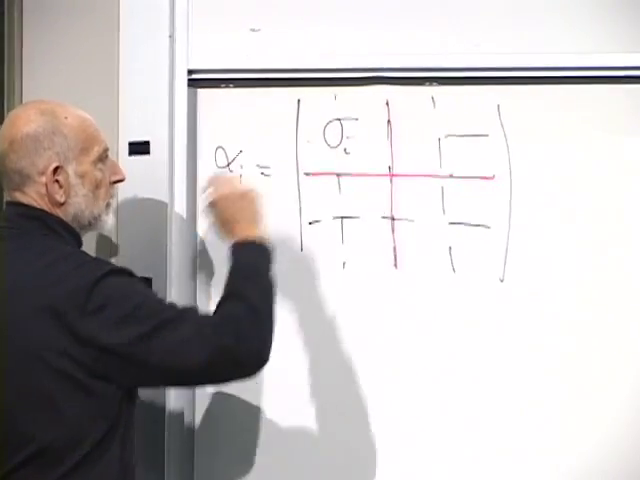
\includegraphics[width=0.68\textwidth]{lecture_08_figure_05.png}
\caption{مصفوفة ديراك \(\alpha_i\) مكتوبة على هيئة كتل \(2\times2\)، مع \(\sigma_i\) و \(-\sigma_i\) على القطر.}
\lectureframe{01:17:23}
\end{figure}

\begin{classroomqa}
\lecturetimestamp{01:17:41}
\audiencequestion{هل كانت كتل \(\sigma_i\) مرتبة على النحو المعاكس في التمثيل السابق؟}
\lecturerresponse{نعم. فقد وُضعت خارج القطر في تمثيل آخر. والترتيبان متكافئان، ويرتبط أحدهما بالآخر بتحويل تشابه.}
\end{classroomqa}

في التمثيل الحالي تكون المصفوفة المتبقية هي
\begin{equation}
\beta=
\begin{pmatrix}
0&I_2\\
I_2&0
\end{pmatrix},
\qquad
I_2=
\begin{pmatrix}
1&0\\
0&1
\end{pmatrix}.
\end{equation}
ويختزل ضرب الكتل التحقق من جبر \(4\times4\) إلى ضرب اعتيادي لمصفوفات \(2\times2\).

\begin{classroomqa}
\lecturetimestamp{01:19:17}
\audiencequestion{هل استخدم التمثيل السابق إشارة مختلفة أو شكلًا قطريًا لـ \(\beta\)؟}
\lecturerresponse{لقد استخدم أساسًا مختلفًا لكنه مكافئ فيزيائيًا. ويخلط تغيير الأساس المركبات الأربع لـ \(\Psi\) ويغيّر مظهر المصفوفات من غير أن يغيّر الفيزياء.}
\end{classroomqa}

المركبات الأربع لـ \(\Psi\) ليست هي الإحداثيات الأربع للزمكان. بل هي إحداثيات في أصغر فضاء متجهي يمكن أن يؤثر عليه جبر مضادات التبديل هذا. وهناك بنيتان ثنائيتان متميزتان: التقسيم إلى كتل \(2\times2\)، والبنية الباولية ثنائية المركبة داخل كل كتلة. واستباقًا للتفسير الذي سيثبت أدناه، يمكن تنظيم الإمكانات الأربع على الصورة
\begin{equation}
\begin{array}{c|cc}
& S_z=+\tfrac12 & S_z=-\tfrac12\\ \hline
\omega>0 & (\omega>0,+\tfrac12) & (\omega>0,-\tfrac12)\\
\omega<0 & (\omega<0,+\tfrac12) & (\omega<0,-\tfrac12)
\end{array}.
\end{equation}
ويتألف الصف السفلي من حالات إلكترون ذات تردد سالب. وهو ليس صفًا من البوزيترونات؛ فسيُفسَّر البوزيترون على أنه ثقب في المجموعة الممتلئة من تلك الحالات.

\section{تضاعف الطاقة في إطار السكون والبوزيترون}

أسهل ما يكون إظهار البنية الثنائية للطاقة عند انعدام الزخم. فعندما يكون \(\mathbf{k}=0\)، تكون حالة الموجة المستوية ثابتة مكانيًا ويختفي حد المشتقة المكانية. ومعادلة إطار السكون\footnote{تحتفظ الشريحة عند \(01{:}23{:}38\) مؤقتًا بعامل إضافي هو \(i\) في حد الكتلة؛ ويزيله التصحيح المنطوق عند \(01{:}24{:}05\).} هي
\begin{equation}
i\frac{\partial\Psi}{\partial t}=m\beta\Psi.
\end{equation}

\begin{figure}[t]
\centering
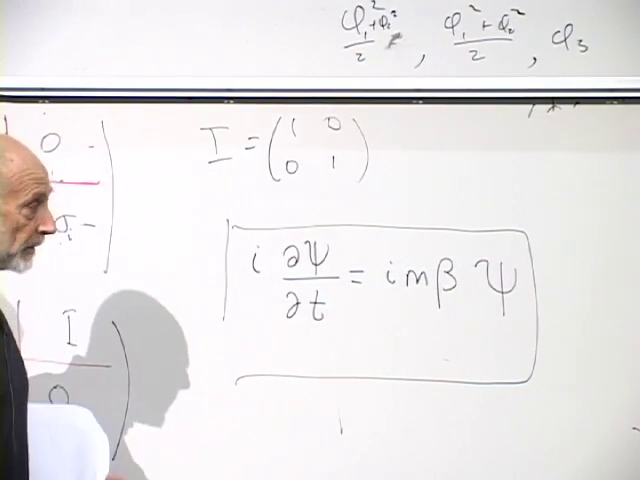
\includegraphics[width=0.76\textwidth]{lecture_08_figure_06.png}
\caption{عند انعدام الزخم تنعدم المشتقات المكانية، فتبقى معادلة إطار السكون المصححة \(i\partial_t\Psi=m\beta\Psi\).}
\lectureframe{01:23:38}
\end{figure}

قسّم العمود ذا المركبات الأربع إلى جزأين، علوي وسفلي، لكل منهما مركبتان:
\begin{equation}
\Psi=
\begin{pmatrix}
\psi_+\\
\psi_-
\end{pmatrix}.
\end{equation}

\begin{classroomqa}
\lecturetimestamp{01:24:47}
\audiencequestion{هل تعني التسميتان \(\psi_+\) و \(\psi_-\) بالفعل الطاقة الموجبة والطاقة السالبة؟}
\lecturerresponse{لا. ففي هذه المرحلة هما مجرد اسمين للكتلتين العلوية والسفلية ثنائيتَي المركبات. ولم تُستخرج تراكيبهما الطاقية بعد.}
\end{classroomqa}

\begin{classroomqa}
\lecturetimestamp{01:25:10}
\audiencequestion{ماذا يمثل العمود المقسَّم ذو المركبات الأربع؟}
\lecturerresponse{إنه السبينور الديراكي نفسه ذو المركبات الأربع، منظَّمًا بحيث يطابق صيغة الكتل للمصفوفات. وكل نصف هو عنصر ذو مركبتين، وعنصران كهذان يكوِّنان العمود الأصلي ذا المركبات الأربع.}
\end{classroomqa}

تبدّل المصفوفة \(\beta\) الكتلتين:
\begin{equation}
\beta
\begin{pmatrix}
\psi_+\\
\psi_-
\end{pmatrix}
=
\begin{pmatrix}
\psi_-\\
\psi_+
\end{pmatrix}.
\end{equation}
ولذلك تصبح معادلة إطار السكون
\begin{equation}
i\frac{\partial\psi_+}{\partial t}=m\psi_-,
\qquad
i\frac{\partial\psi_-}{\partial t}=m\psi_+.
\end{equation}

هناك اقتراحان طبيعيان. فأخذ مشتقة زمنية أخرى من شأنه أن يفصل النظام، لكن جمع المعادلتين وطرحهما يجعلهما في صورة قطرية فورًا. وفي الواقع،
\begin{align}
i\frac{\partial}{\partial t}(\psi_++\psi_-)
&=m(\psi_++\psi_-),\\
i\frac{\partial}{\partial t}(\psi_+-\psi_-)
&=-m(\psi_+-\psi_-).
\end{align}
وبتعريف
\begin{equation}
\chi_+=\psi_++\psi_-,
\qquad
\chi_-=\psi_+-\psi_-,
\end{equation}
نحصل على معادلتين مستقلتين،
\begin{equation}
i\partial_t\chi_+=m\chi_+,
\qquad
i\partial_t\chi_-=-m\chi_-.
\end{equation}
وبالنسبة إلى اعتماد ذي تردد محدد \(e^{-i\omega t}\)، يكون للمجموع
\begin{equation}
\omega=+m,
\end{equation}
بينما يكون للفرق
\begin{equation}
\omega=-m.
\end{equation}
وهذا هو بالضبط تضاعف الطاقة الموجبة والسالبة الذي وُجد في المثال الأحادي البعد السابق: فالمعادلة النسبية تمتلك مرة أخرى حلول إلكترون ذات طاقة موجبة وحلول إلكترون ذات طاقة سالبة. ومن ثم ينفصل تضاعف الكتل إلى فرعين للطاقة الموجبة والسالبة. ويمكن كتابة حالات إطار السكون الخالصة على الصورة
\begin{equation}
\Psi_{\omega=+m}=
\begin{pmatrix}
\xi\\
\xi
\end{pmatrix},
\qquad
\Psi_{\omega=-m}=
\begin{pmatrix}
\xi\\
-\xi
\end{pmatrix},
\end{equation}
حيث تظل \(\xi\) عنصرًا اعتباطيًا ذا مركبتين.

لقد تخلَّص المجموع والفرق من إحدى البنيتين الثنائيتين، لكن المركبتين في \(\xi\) تبقيان. وتؤثر مصفوفات باولي في هذا الزوج المتبقي. وهذا هو الزوج المرتبط باللف المغزلي، والخاضع للتحقق المتعلق بالدوران وقانون الانحفاظ الذي سيُناقش أدناه.

\begin{classroomqa}
\lecturetimestamp{01:32:23}
\audiencequestion{هل يمكن التعامل مع اللف المغزلي بوصفه البنية الثنائية الخارجية، ومع إشارة الطاقة بوصفها الداخلية؟}
\lecturerresponse{نعم. إن ترتيبي العاملين متكافئان. ويمكن تبديل أي الفهرسين يُكتب أولًا؛ فالتغيير ليس إلا إعادة ترتيب للمركبات الأربع.}
\end{classroomqa}

يقود فرع التردد السالب إلى تفسير بحر ديراك. ويُسنَد إلى التردد السالب طاقة إلكترون سالبة. وملء كل حالة إلكترون سالبة الطاقة يخفِّض الطاقة إلى أبعد مدى يسمح به مبدأ الاستبعاد، لأن إلكترونًا واحدًا فقط يمكنه أن يشغل كل حالة فيرميونية كاملة. وعندئذ يُسمَّى بحر الطاقة السالبة الممتلئ تمامًا الفراغ.

انقل إلكترونًا واحدًا من هذا البحر المملوء إلى حالة موجبة الطاقة. تحتوي النتيجة على إلكترون ذي طاقة موجبة وعلى حالة سالبة الطاقة غير مشغولة. إن إزالة طاقة سالبة ترفع الطاقة، لذا تكون للفجوة طاقة إثارة موجبة؛ ولأن إلكترونًا مفقود، فإنها تحمل أيضًا الشحنة الكهربائية المعاكسة. الفجوة هي بوزيترون.

\begin{classroomqa}
\lecturetimestamp{01:32:57}
\audiencequestion{هل يمكن شرح تفسير البوزيترون مرة أخرى؟}
\lecturerresponse{مجموع الجزأين له تردد موجب وفرقُهما له تردد سالب. وحلول التردد السالب هي حالات إلكترون سالبة الطاقة، ويُحصَل على الفراغ بملء جميعها. إن رفع أحد الإلكترونات المشغولة إلى طاقة موجبة يترك إلكترونًا ذا طاقة موجبة وفجوةً معًا. وتلك الفجوة ذات الطاقة الموجبة والشحنة المعاكسة هي البوزيترون.}
\end{classroomqa}

وهكذا أنتج الجبر في آن واحد نتيجتين: فرعي الطاقة الموجبة والسالبة، اللذين يصبحان بنية الجسيم--ضد الجسيم، وبنيةً متبقيةً ذات مركبتين مرتبطة بلف مغزلي مقداره نصف. والنقطة اللافتة هي أن كليهما انبثق من أصغر المصفوفات القادرة على استيفاء علاقات ضديد التبديل النسبية. ولم يكن اللف المغزلي قد ظهر إلا حديثًا بوصفه خاصية تجريبية حين أنتج هذا البناء الرياضي جسيماتٍ ذات لف مغزلي مع فرعٍ لضد الجسيم؛ وفي ذلك السياق التاريخي كانت النتيجة مثيرة.

\begin{classroomqa}
\lecturetimestamp{01:35:14}
\audiencequestion{هل الإلكترونات سالبة الطاقة نفسها هي البوزيترونات؟}
\lecturerresponse{لا. حالات الإلكترون سالبة الطاقة مملوءة في الفراغ. والبوزيترون هو غياب إلكترون واحد من تلك المجموعة المملوءة: فجوة، لا إلكترون سالب الطاقة.}
\end{classroomqa}

يمكن للفجوة أن تشارك في انتقالات. وللبوزيترون طاقة موجبة لأنه غياب إلكترون سالب الطاقة. وإذا ملأ إلكترون ذو طاقة موجبة الفجوة، فإن الإلكترون والبوزيترون يفني أحدهما الآخر، ولكن لا بد أن تُحمَل طاقتهما بعيدًا، عادةً بواسطة الفوتونات. وبلغة البحر، يكون إلكترون قد ملأ حالة سالبة الطاقة غير مشغولة. ويمكن تصوير انطلاق الطاقة نفسه كما لو أن إلكترونًا مثارًا في ذرة يهبط إلى مستوى أدنى: فالانتقال الهابط يبعث فوتونات.

\begin{classroomqa}
\lecturetimestamp{01:36:39}
\audiencequestion{لماذا لا تهبط الإلكترونات الواقعة عند طاقات سالبة أعلى إلى الفجوة؟}
\lecturerresponse{هذا السؤال يخلط بين حالتين. فملء الفجوة بإلكترون ذي طاقة موجبة هو إفناء إلكترون--بوزيترون، مع حمل الفوتونات للطاقة بعيدًا. أما انتقال إلكترون من بحر الطاقات السالبة فهو عملية مختلفة، ستُتناول أدناه.}
\end{classroomqa}

إن حساب الزخم الصفري، بمفرده، قد أثبت انحلالًا ثنائيًا بعد فصل إشارة الطاقة. لكن وجود انحلال بين حالتين ليس، بمفرده، برهانًا على أن هاتين الحالتين تحملان زخمًا زاويًا.

\begin{classroomqa}
\lecturetimestamp{01:37:44}
\audiencequestion{كيف يثبت حساب الزخم الصفري أن الزوج المتبقي من الحالات يمثل لفًا مغزليًا؟}
\lecturerresponse{يمكن تسمية هذا الزوج أعلى وأسفل، وتظهر مصفوفات باولي في المعادلة الكاملة، لكن ذلك وحده ليس برهانًا بعد. فلا بد إما من إظهار كيف يتحول الزوج تحت الدورانات المكانية، أو من أن إسناد لف مغزلي إليه يجعل الزخم الزاوي الكلي محفوظًا في التفاعلات والتصادمات. ويُؤجَّل هذا البرهان.}
\end{classroomqa}

بالنسبة إلى حالة سكون موجبة الطاقة، يكون الجزآن العلوي والسفلي متساويين،
\begin{equation}
\Psi_{\omega=+m}=
\begin{pmatrix}
\xi\\
\xi
\end{pmatrix}.
\end{equation}
وأما إثبات أن \(\xi\) يشكل مزدوجة زخم زاوي، فيتطلب حجة الدوران أو الانحفاظ التي وُصفت للتو؛ ولا يترتب ذلك لمجرد عد مركبتين.

\begin{classroomqa}
\lecturetimestamp{01:40:46}
\audiencequestion{هل يمكن لإلكترون مختلف أن يفنى مع البوزيترون حتى لو كانت طاقته مختلفة؟}
\lecturerresponse{نعم. لا تحتفظ الإلكترونات بأي هوية فردية. ويمكن لأي إلكترون متاح أن يملأ الفجوة، وتنعكس الفروق في الطاقة والزخم الابتدائيين في عدد الفوتونات المنبعثة وطاقاتها.}
\end{classroomqa}

كما تفسر صورة الفجوة أيضًا انتقالًا يقع بأكمله داخل بحر الطاقات السالبة. افترض أن حالة سالبة الطاقة مشغولة انتقلت إلى الفجوة. عندئذٍ تُملأ الفجوة الأصلية، لكن الحالة التي جاء منها ذلك الإلكترون تصبح الآن فارغة. لقد انتقلت الفجوة. وبصورة مكافئة، يكون البوزيترون قد غيّر طاقته وأصدر إشعاعًا.

\begin{classroomqa}
\lecturetimestamp{01:42:12}
\audiencequestion{لماذا لا يمكن للمستويات سالبة الطاقة المجاورة أن تهبط تباعًا إلى الفجوة؟}
\lecturerresponse{يمكنها أن تنقل الفجوة من مستوى إلى آخر. فإلكترون يهبط إلى الفجوة القديمة يترك فجوة جديدة عند طاقته السابقة، ولذلك يصبح البوزيترون الابتدائي بوزيترونًا ذا طاقة مختلفة. وتحمل الفوتونات فرق الطاقة.}
\end{classroomqa}

\begin{classroomqa}
\lecturetimestamp{01:44:39}
\audiencequestion{لماذا لا يؤدي هذا إلى شلالٍ إشعاعي هابط بلا نهاية؟}
\lecturerresponse{لأن الطاقة والزخم يجب أن يُحفَظا في آن واحد. وهذان قانونا الانحفاظ لا يسمحان بهذه العملية غير المقيّدة. وتنشأ المسألة نفسها بالنسبة إلى إلكترون حر عادي: إذ لا يمكنه ببساطة أن يواصل خفض طاقته بإصدار فوتونات في الفضاء الخالي.}
\end{classroomqa}